\section{Subespacios vectoriales}

\subsection{}

\begin{frame}\frametitle{Subespacio vectorial}

%\begin{exampleblock}{\textbf{Definición 2}}
\begin{block}{\textbf{Definición 1 (Subespacio vectorial)}}	
	\justifying
	Un subconjunto no vacío $W$ de un espacio vectorial $V$ se dice que es un {\color{red} subespacio (vectorial)} 
	de $V$, si $W$ es un espacio vectorial bajo las operaciones de \textit{suma} y \textit{multiplicación por escalar} definidas en $V$.
\end{block}


\begin{alertblock}{\textbf{Observación 1}}\justifying
	Si $W$ es un subespacio de $V$, entonces $W$ debe ser cerrado bajo las operaciones inherentes a $V$.
\end{alertblock}

\end{frame}

%%------------------------------------------------------------------------------------------------------

\subsection{}

\begin{frame}%\frametitle{Ejemplo}

%\begin{exampleblock}{\textbf{Definición 2}}
\begin{block}{\textbf{Definición 1 (Subespacio vectorial)}}	
	\justifying
	Un subconjunto no vacío $W$ de un espacio vectorial $V$ se dice que es un {\color{red} subespacio (vectorial)} 
	de $V$, si $W$ es un espacio vectorial bajo las operaciones de \textit{suma} y \textit{multiplicación por escalar} definidas en $V$.
\end{block}

\begin{ej}{\textbf{Ejemplo 1}}\justifying
	Demuestre que el conjunto 
	\[
		W = \{ (x_1,0,x_3) \mid x_1 \text{ y } x_3 \ \text{ son números reales } \}
	\]
	es un \textit{subespacio} de $\r^3$ con las operaciones usuales.
\end{ej}

\begin{figure}	
	\begin{subfigure}[b]{\textwidth}
		\centering
		\begin{tikzpicture} [x={(-0.6cm,-0.4cm)}, y={(1cm,0cm)}, z={(0cm,1cm)},scale=1, every node/.style={scale=0.8}]
			\begin{scope}[canvas is yx plane at z=0]
	%		\draw[orange,thick] (2,2) circle (1cm);
			%\draw [orange!30] (0,0) grid (1,1);   
			\draw [black,line width=0.3mm,->] (0,0) -- (3,1.5)node[below,right] {$y$};  
			\draw [black,line width=0.3mm,->] (0,0) -- (0,3)node[left] {$x$}; 
			%\draw[top color=orange!30,fill opacity=.5,orange] (3,0)--(3,3)--(0,2)--cycle;   
			\end{scope}
			%
			\begin{scope}[canvas is zx plane at y=0]
			%\draw[blue,thick] (2,2) circle (1cm);			
			\draw [black,line width=0.3mm,->] (0,0) -- (2,0) node[above,right] {$z$};
			\fill[color=blue,draw] (1.5,2) circle (2pt) node[above] {$(x_1,0,x_3)$};
			\draw [blue,line width=0.2mm,->] (0,0) -- (1.5,2);% node[above] {$(x_1,0,x_3)$};
			\fill[color=blue,draw] (0.8,1) node[above] { $\u$};	
			\draw [blue!30] (0,0) grid (2,3); 
			%\draw[top color=blue!30,fill opacity=.5,blue] (3,0)--(3,3)--(0,2)--cycle;       
			\end{scope}
			
		\end{tikzpicture}   
		% \caption{${\color{blue}f}, {\color{verde}0.5f}, {\color{red}1.5f}$}
	\end{subfigure}	
	%	\caption{Pictures of animals}\label{fig:animals}
\end{figure}

\end{frame}

%%------------------------------------------------------------------------------------------------------

\subsection{}

{\nologo
\begin{frame}\frametitle{Prueba para un subespacio}

\vspace{-2mm}

%\begin{exampleblock}{\textbf{Definición 2}}
\begin{block}{\textbf{Definición 1 (Subespacio vectorial)}}	
	\justifying
	Un subconjunto no vacío $W$ de un espacio vectorial $V$ se dice que es un {\color{red} subespacio (vectorial)} 
	de $V$, si $W$ es un espacio vectorial bajo las operaciones de \textit{suma} y \textit{multiplicación por escalar} definidas en $V$.
\end{block}

\begin{prop}{\textbf{Propiedad 1}}
	\justifying
	Un subconjunto no vacío $W$ de un espacio vectorial $V$ es {\color{red} subespacio} 
	de $V$ si y solo si se cumplen las siguientes condiciones:
	\begin{enumerate}
		\item[\labelname{$a$}] Si $\u$ y $\v$ están en $W$, entonces $\u+\v$ está en $W$.
		\item[\labelname{$b$}] Si $\u$ está en $W$ y $c$ es un escalar, entonces $c\u$ está en $W$.
	\end{enumerate}
\end{prop}

\begin{alertblock}{\textbf{Observación 2}}
	\begin{enumerate}\justifying
		\item[\labelname{$a$}] Si $W$ es un subespacio vectorial de $V$, entonces tanto $W$ como $V$ deben 
		tener el mismo vector cero $\mathbf{0}$.
		\item[\labelname{$b$}] El subespacio vectorial  más simple de un espacio vectorial $V$ es $W=\{\mathbf{0}\}$.
		\item[\labelname{$c$}] Otro subespacio vectorial obvio de un espacio vectorial $V$ es $W=V$.
	\end{enumerate}
\end{alertblock}

\end{frame}
}

%%------------------------------------------------------------------------------------------------------

\subsection{}

\begin{frame}\frametitle{Un subespacio de $\r^2$}

\begin{prop}{\textbf{Propiedad 1}}
	\justifying
	Un subconjunto no vacío $W$ de un espacio vectorial $V$ es {\color{red} subespacio} 
	de $V$ si y solo si se cumplen las siguientes condiciones:
	\begin{enumerate}
		\item[\labelname{$a$}] Si $\u$ y $\v$ están en $W$, entonces $\u+\v$ está en $W$.
		\item[\labelname{$b$}] Si $\u$ está en $W$ y $c$ es un escalar, entonces $c\u$ está en $W$.
	\end{enumerate}
\end{prop}

\begin{ej}{\textbf{Ejemplo 2}}\justifying
	Demuestre que el conjunto 
	\[
	W = \{ (x,y) \mid x+2y=0 \}
	\]
	es un \textit{subespacio} de $\r^2$.
\end{ej}

\end{frame}

%%------------------------------------------------------------------------------------------------------

\subsection{}

\begin{frame}\frametitle{Un conjunto que no es subespacio de $\r^2$}

\begin{prop}{\textbf{Propiedad 1}}
	\justifying
	Un subconjunto no vacío $W$ de un espacio vectorial $V$ es {\color{red} subespacio} 
	de $V$ si y solo si se cumplen las siguientes condiciones:
	\begin{enumerate}
		\item[\labelname{$a$}] Si $\u$ y $\v$ están en $W$, entonces $\u+\v$ está en $W$.
		\item[\labelname{$b$}] Si $\u$ está en $W$ y $c$ es un escalar, entonces $c\u$ está en $W$.
	\end{enumerate}
\end{prop}

\begin{ej}{\textbf{Ejemplo 3}}\justifying
	Demuestre que el conjunto 
	\[
	W = \{ (x,y) \mid x+2y=1 \}
	\]
	\textbf{no} es un \textit{subespacio} de $\r^2$.
\end{ej}

\end{frame}

%%------------------------------------------------------------------------------------------------------

\subsection{}

\begin{frame}\frametitle{Un subespacio de $\r^3$}

\begin{prop}{\textbf{Propiedad 1}}
	\justifying
	Un subconjunto no vacío $W$ de un espacio vectorial $V$ es {\color{red} subespacio} 
	de $V$ si y solo si se cumplen las siguientes condiciones:
	\begin{enumerate}
		\item[\labelname{$a$}] Si $\u$ y $\v$ están en $W$, entonces $\u+\v$ está en $W$.
		\item[\labelname{$b$}] Si $\u$ está en $W$ y $c$ es un escalar, entonces $c\u$ está en $W$.
	\end{enumerate}
\end{prop}

\begin{ej}{\textbf{Ejemplo 4}}\justifying
	Demuestre que el conjunto 
	\[
	W = \{ (x,y,z) \mid ax+by+cz = 0, \text{ con } a, b, c \text{ números reales } \}
	\]
	es un \textit{subespacio} de $\r^3$.
\end{ej}

\end{frame}

%%------------------------------------------------------------------------------------------------------

\subsection{}

\begin{frame}\frametitle{Un subespacio de $M_{22}$}

\begin{prop}{\textbf{Propiedad 1}}
	\justifying
	Un subconjunto no vacío $W$ de un espacio vectorial $V$ es {\color{red} subespacio} 
	de $V$ si y solo si se cumplen las siguientes condiciones:
	\begin{enumerate}
		\item[\labelname{$a$}] Si $\u$ y $\v$ están en $W$, entonces $\u+\v$ está en $W$.
		\item[\labelname{$b$}] Si $\u$ está en $W$ y $c$ es un escalar, entonces $c\u$ está en $W$.
	\end{enumerate}
\end{prop}

\begin{ej}{\textbf{Ejemplo 5}}\justifying
	Sea $W$ el conjunto de todas las matrices simétricas de $2\times 2$. Demuestre que $W$  es
	un subespacio de $M_{22}$.
\end{ej}

\end{frame}

%%------------------------------------------------------------------------------------------------------

\subsection{}

\begin{frame}\frametitle{Un conjunto que no es subespacio de $M_{22}$}

\begin{prop}{\textbf{Propiedad 1}}
\justifying
Un subconjunto no vacío $W$ de un espacio vectorial $V$ es {\color{red} subespacio} 
de $V$ si y solo si se cumplen las siguientes condiciones:
\begin{enumerate}
	\item[\labelname{$a$}] Si $\u$ y $\v$ están en $W$, entonces $\u+\v$ está en $W$.
	\item[\labelname{$b$}] Si $\u$ está en $W$ y $c$ es un escalar, entonces $c\u$ está en $W$.
\end{enumerate}
\end{prop}

\begin{ej}{\textbf{Ejemplo 6}}\justifying
Sea $W$ el conjunto de todas las matrices singulares de $2\times 2$. Demuestre que $W$ \textbf{no} es
un subespacio de $M_{22}$.
\end{ej}

\end{frame}

%%------------------------------------------------------------------------------------------------------

\subsection{}

\begin{frame}\frametitle{Subespacios de funciones}

\begin{ej}{\textbf{Ejemplo 7}}\justifying
	Sea $\mathcal{C}$ el conjunto de todas las funciones continuas de valor real definidas en $\r$ y
	sea $\mathcal{D}$ el conjunto de todas las funciones derivables de valor real definidas en $\r$.
	Demuestre que $\mathcal{C}$ y $\mathcal{D}$ son subespacios vectoriales de $\mathcal{F}$, el 
	espacio vectorial de todas las funciones con valor real definidas en $\r$.
\end{ej}

\begin{figure}	
	\begin{subfigure}[b]{\textwidth}
		\centering
		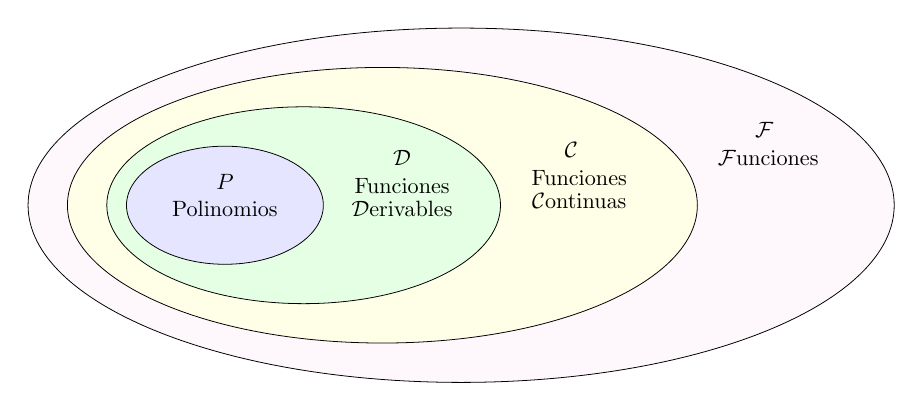
\begin{tikzpicture}[thick,scale=0.5, every node/.style={scale=0.8}]
			% F
			\draw[line width=0.1mm,fill=magenta!3]    (0,0) ellipse (11cm and 4.5 cm);
			\fill[color=black,draw] (7.7,1.5) node[above] { $\mathcal{F}$};	
			\fill[color=black,draw] (7.8,0.8) node[above] {$\mathcal{F}$unciones};	
			% C
			\draw[line width=0.1mm,fill=yellow!10] (-2,0) ellipse (8cm and 3.5 cm);
			\fill[color=black,draw] (2.8,1) node[above] { $\mathcal{C}$};
			\fill[color=black,draw] (3,0.3) node[above] {Funciones};
			\fill[color=black,draw] (3,-0.3) node[above] {$\mathcal{C}$ontinuas};
			% D
			\draw[line width=0.1mm,fill=white!90!green]  (-4,0) ellipse  (5cm and 2.5 cm);	
			\fill[color=black,draw] (-1.5,0.8) node[above] { $\mathcal{D}$};	
			\fill[color=black,draw] (-1.5,0.1) node[above] {Funciones};
			\fill[color=black,draw] (-1.5,-0.5) node[above] {$\mathcal{D}$erivables};
			% P
			\draw[line width=0.1mm,fill=white!90!blue]  (-6,0) ellipse  (2.5cm and 1.5 cm);	
			\fill[color=black,draw] (-6,0.2) node[above] { $P$};
			\fill[color=black,draw] (-6,-0.5) node[above] {Polinomios};
		\end{tikzpicture} 
		\caption{$P\subseteq \mathcal{D}\subseteq \mathcal{C}\subseteq \mathcal{F}$}
	\end{subfigure}	
	%	\caption{Pictures of animals}\label{fig:animals}
\end{figure}

\end{frame}

%%------------------------------------------------------------------------------------------------------

\subsection{}

{\nologo
\begin{frame}\frametitle{Intersección de subespacios}

\begin{prop}{\textbf{Propiedad 2}}
	\justifying
	Si $V$ y $W$ son subespacios de un espacio vectorial $U$, entonces la intersección de $V$ y $W$,
	denotada por $V\cap W$, también es un subespacio de $U$.
\end{prop}

\begin{figure}	
	\begin{subfigure}[b]{\textwidth}
		\centering
		% Definition of circles
		%\def\firstcircle{(0,0) circle (1.5cm)}
		\def\firstcircle{(0,0) ellipse (2cm and 1.5 cm)}
		%\def\secondcircle{(0:2cm) circle (1.5cm)}		
		\def\secondcircle{(0:2cm) ellipse (2cm and 1.5 cm)}		
		\colorlet{circle edge}{blue!50}
		\colorlet{circle area}{blue!20}		
		\tikzset{filled/.style={fill=circle area, draw=circle edge},
			outline/.style={draw=circle edge}}		
		\setlength{\parskip}{5mm}
		% Set A and B
		\begin{tikzpicture}[thick,scale=0.8, every node/.style={scale=0.8}]
			\begin{scope}
				\clip \firstcircle;
				\fill[filled] \secondcircle;
			\end{scope}
			\draw[outline] \firstcircle node at (-1,0) {$V$};
			\draw[outline] \secondcircle node at (3,0) {$W$};
			%\node[anchor=south] at (current bounding box.north) {$A \cap B$};
			\node[anchor=south] at (1,-0.2) {$V \cap W$};
			\draw[line width=0.1mm] (-3,-2) rectangle (5,2) node [text=black,above] {$U$};
		\end{tikzpicture}		
		\caption{La intersección de subespacios es subespacio}
	\end{subfigure}	
	%	\caption{Pictures of animals}\label{fig:animals}
\end{figure}

\begin{alertblock}{\textbf{Observación 3}}
	La unión de subespacios \textbf{no} es (en general) un subespacio.
\end{alertblock}

\end{frame}
}

%%------------------------------------------------------------------------------------------------------

\subsection{}

\begin{frame}\frametitle{Intersección de subespacios}

\begin{prop}{\textbf{Propiedad 2}}
	\justifying
	Si $V$ y $W$ son subespacios de un espacio vectorial $U$, entonces la intersección de $V$ y $W$,
	denotada por $V\cap W$, también es un subespacio de $U$.
\end{prop}

\begin{ej}{\textbf{Ejemplo 8}}\justifying
	En $\r^3$ considere los conjuntos
	\[
		V = \{ (x,y,z) \mid x+2y+3z = 0 \}
	\]
	y
	\[
		W = \{ (x,y,z) \mid  2x-y-z = 0 \}.
	\]
	Demuestre que $V\cap W$ es un subespacio de $\r^3$. Describa a dicho subespacio.
\end{ej}

\end{frame}
